\documentclass[12pt,a4paper]{beamer}
%\usepackage[utf8x]{inputenc}
%\usepackage{ucs}
\usepackage{amsmath}
\usepackage{amsfonts}
\usepackage{amssymb}
\usepackage{graphicx}
\usepackage{wrapfig}
\usepackage{verbatim}
\usepackage{xcolor}

\author{Robin Ellerkmann, Sven Reber}
\title{Konflikthandhabung\\Theorie und Praxis}

\begin{document}
\maketitle

\begin{frame}
	\frametitle{Inhalt}
	
	% FIXME: am Ende noch mal dem "echten" Inhalt/Titeln anpassen.
	\begin{itemize}
		\item Einleitung und Definition eines Konfliktes		% Sven
		\item Vergleich der Modelle					% Robin
		\begin{itemize}
			\item Prozessmodell
			\item Strukturmodell
		\end{itemize}
		\item F\"uhrungsstile							% Sven (ersten 3), Robin (widh-drawing, inaction)
		% XXX: F?r den Inahlt vllt. doch etwas zu viel/fr?h. "Erschl?t" vllt. etwas. (Sven)		
		%\begin{itemize}
		%	\item Vermeidung (in-action)				% Robin
		%	\item Machteinsatz						% Sven
		%	\item Kompromiss						% Sven
		%	\item Anpassung (with-drawing)				% Robin
		%	\item Zusammenarbeit (problem solving)		% Sven
		%\end{itemize}
		\item Fazit									% Robin (?)
	\end{itemize}
\end{frame}

\begin{frame}
	\frametitle{Modelle der Konflikthandhabung}
	\begin{itemize}
		\item Modellieren Konfliktverhalten zwischen zwei Parteien
		\item Zwei Ans�tze:
		\begin{itemize}
			\item Prozessmodell
			\item Strukturmodell
		\end{itemize}
	\end{itemize}
\end{frame}

\begin{frame}
	\frametitle{Prozessmodell}
	\begin{itemize}
		\item Beschreibt interne Dynamik eines Konflikt als Ablauf von Phasen
		\item Events identifizieren und deren Bedeutung für weitere Events ermitteln
		\item Dyadische Konflikte laufen in Eventzyklen ab
	\end{itemize}
\end{frame}

\begin{frame}
	\frametitle{Abbildung Prozessmodell}
	\begin{figure}[p]
    		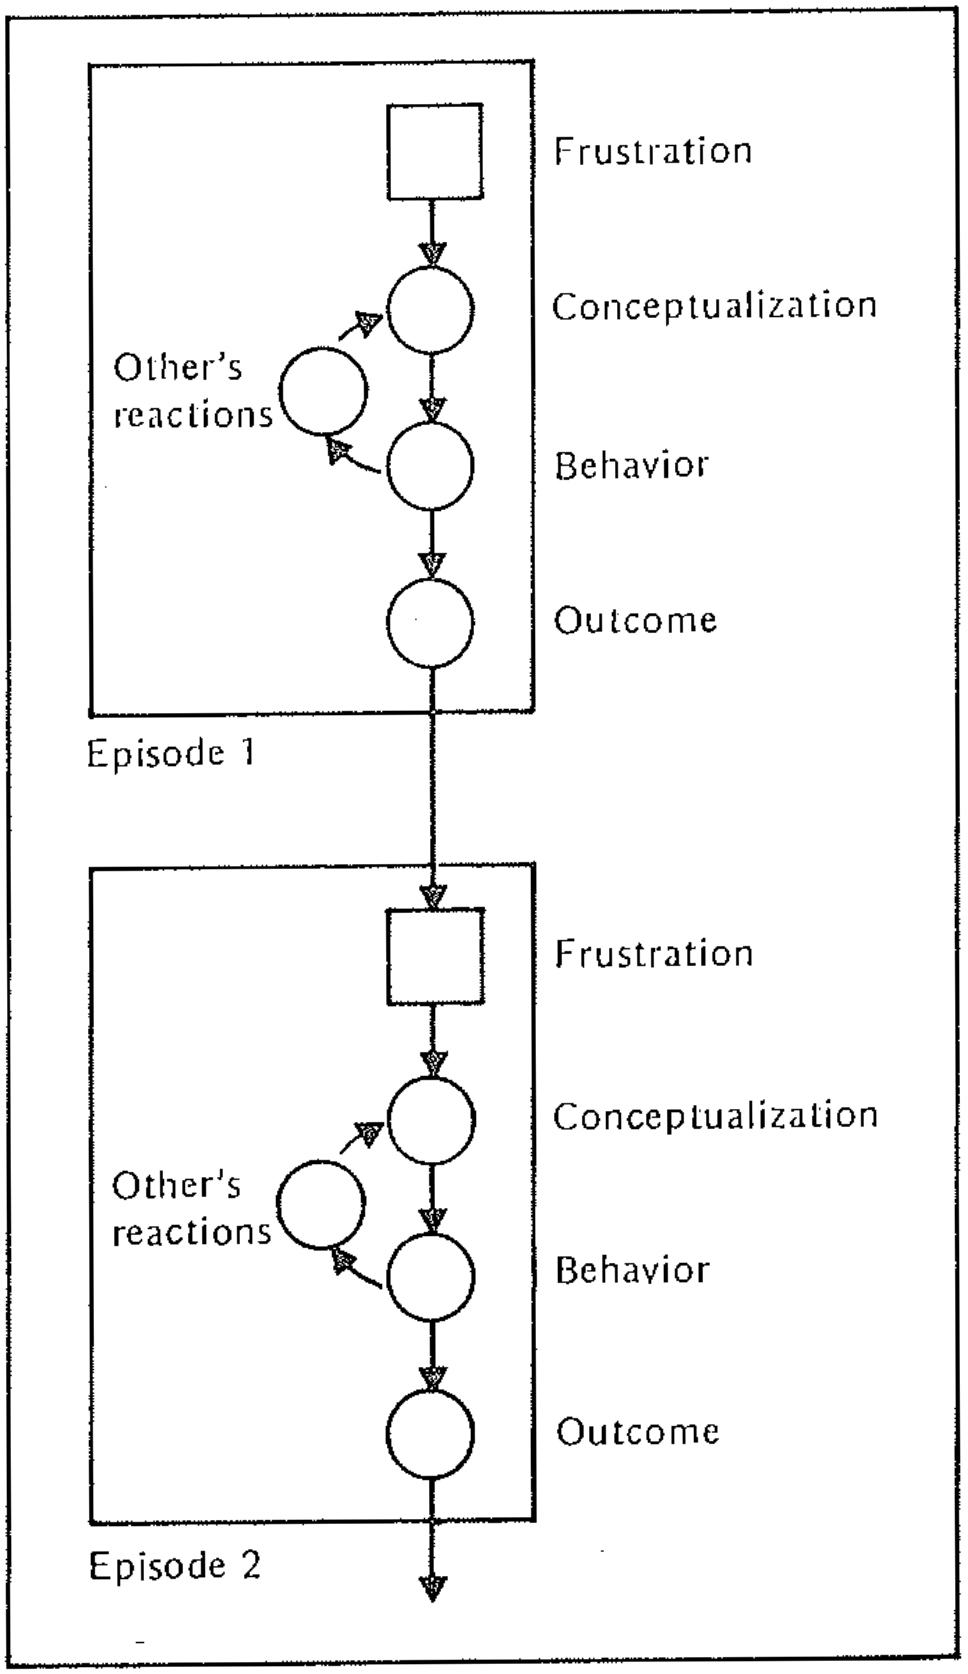
\includegraphics[width=0.4\textwidth]{images/process_model.png}
	\end{figure}
\end{frame}

\begin{frame}
	\frametitle{Frustration}
	\begin{itemize}
		\item Ausgangspunkt für Konflikte: Frustration bei einer der Parteien
		\item Frustration kann viele Formen haben
	\end{itemize}
\end{frame}

\begin{frame}
%//TODO: Adjust name
	\frametitle{Wahrnehmung}
	\begin{itemize}
		\item Subjektive Definition des Anliegens für beide Parteien
		\item Drei Dimensionen bestimmen diese Definition:
		\begin{itemize}
			\item Egozentrik
			\item Einblick in zugrundeliegende Belange
			\item Größe/Wichtigkeit des Problems
		\end{itemize}
		\item Bewusstsein über mögliche Handlungen und deren Folgen ist begrenzt
	\end{itemize}
\end{frame}

\begin{frame}
	\frametitle{Verhalten}
	\begin{itemize}
		\item Besteht aus drei Komponenten: Orientierung, strategische Ziele und Taktiken
		\item Orientierung: Wie wichtig ist einer Partei die Erfüllung des eigenen Anliegens? Wie wichtig ist die Erfüllung des Anliegens der anderen Partei?
		\item Strategische Ziele: Anpassung der Verhaltensweisen an den Gegenüber
		\item Taktiken: Beschreiben bestimmte Verhaltensweisen der Parteien. Z.B als Wettbewerbstaktik, Kooperative Taktik, Bargaining Taktik
	\end{itemize}
\end{frame}

\begin{frame}
	\frametitle{Interaktion}
	\begin{itemize}
		\item Zwei Perspektiven: Verhaltensweisen sind selbst gewählt oder Verhaltensweisen werden durch Aktionen der anderen Partei ausgelöst
		\item Selbst gewähltes Verhalten: Veränderung der Wahrnehmung des Konflikts ändert Verhalten
		\item Ausgelöstes Verhalten: Resultiert aus psychologischen Dynamiken, z.B. Eskalation/Deeskalation
	\end{itemize}
\end{frame}

\begin{frame}
	\frametitle{Ergebnis}
	\begin{itemize}
		\item Nachwirkungen des Konflikts
		\item Langzeiteffekte 
	\end{itemize}
\end{frame}

\begin{frame}
	\frametitle{Strukturmodell}
	\begin{itemize}
		\item Identifiziert Parameter, die das Konfliktverhalten der Parteien beeinflussen
		\item Drei Arten von Einfluss auf das Konfliktverhalten jeder Partei:
		\begin{itemize}
			\item Verhaltensabsichten der Partei
			\item Sozialer Druck auf die Partei
			\item Beziehung zwischen den Interessen der Parteien
		\end{itemize}
	\end{itemize}
\end{frame}

\begin{frame}
	\frametitle{Abbildung Strukturmodell}
	\begin{figure}[p]
    		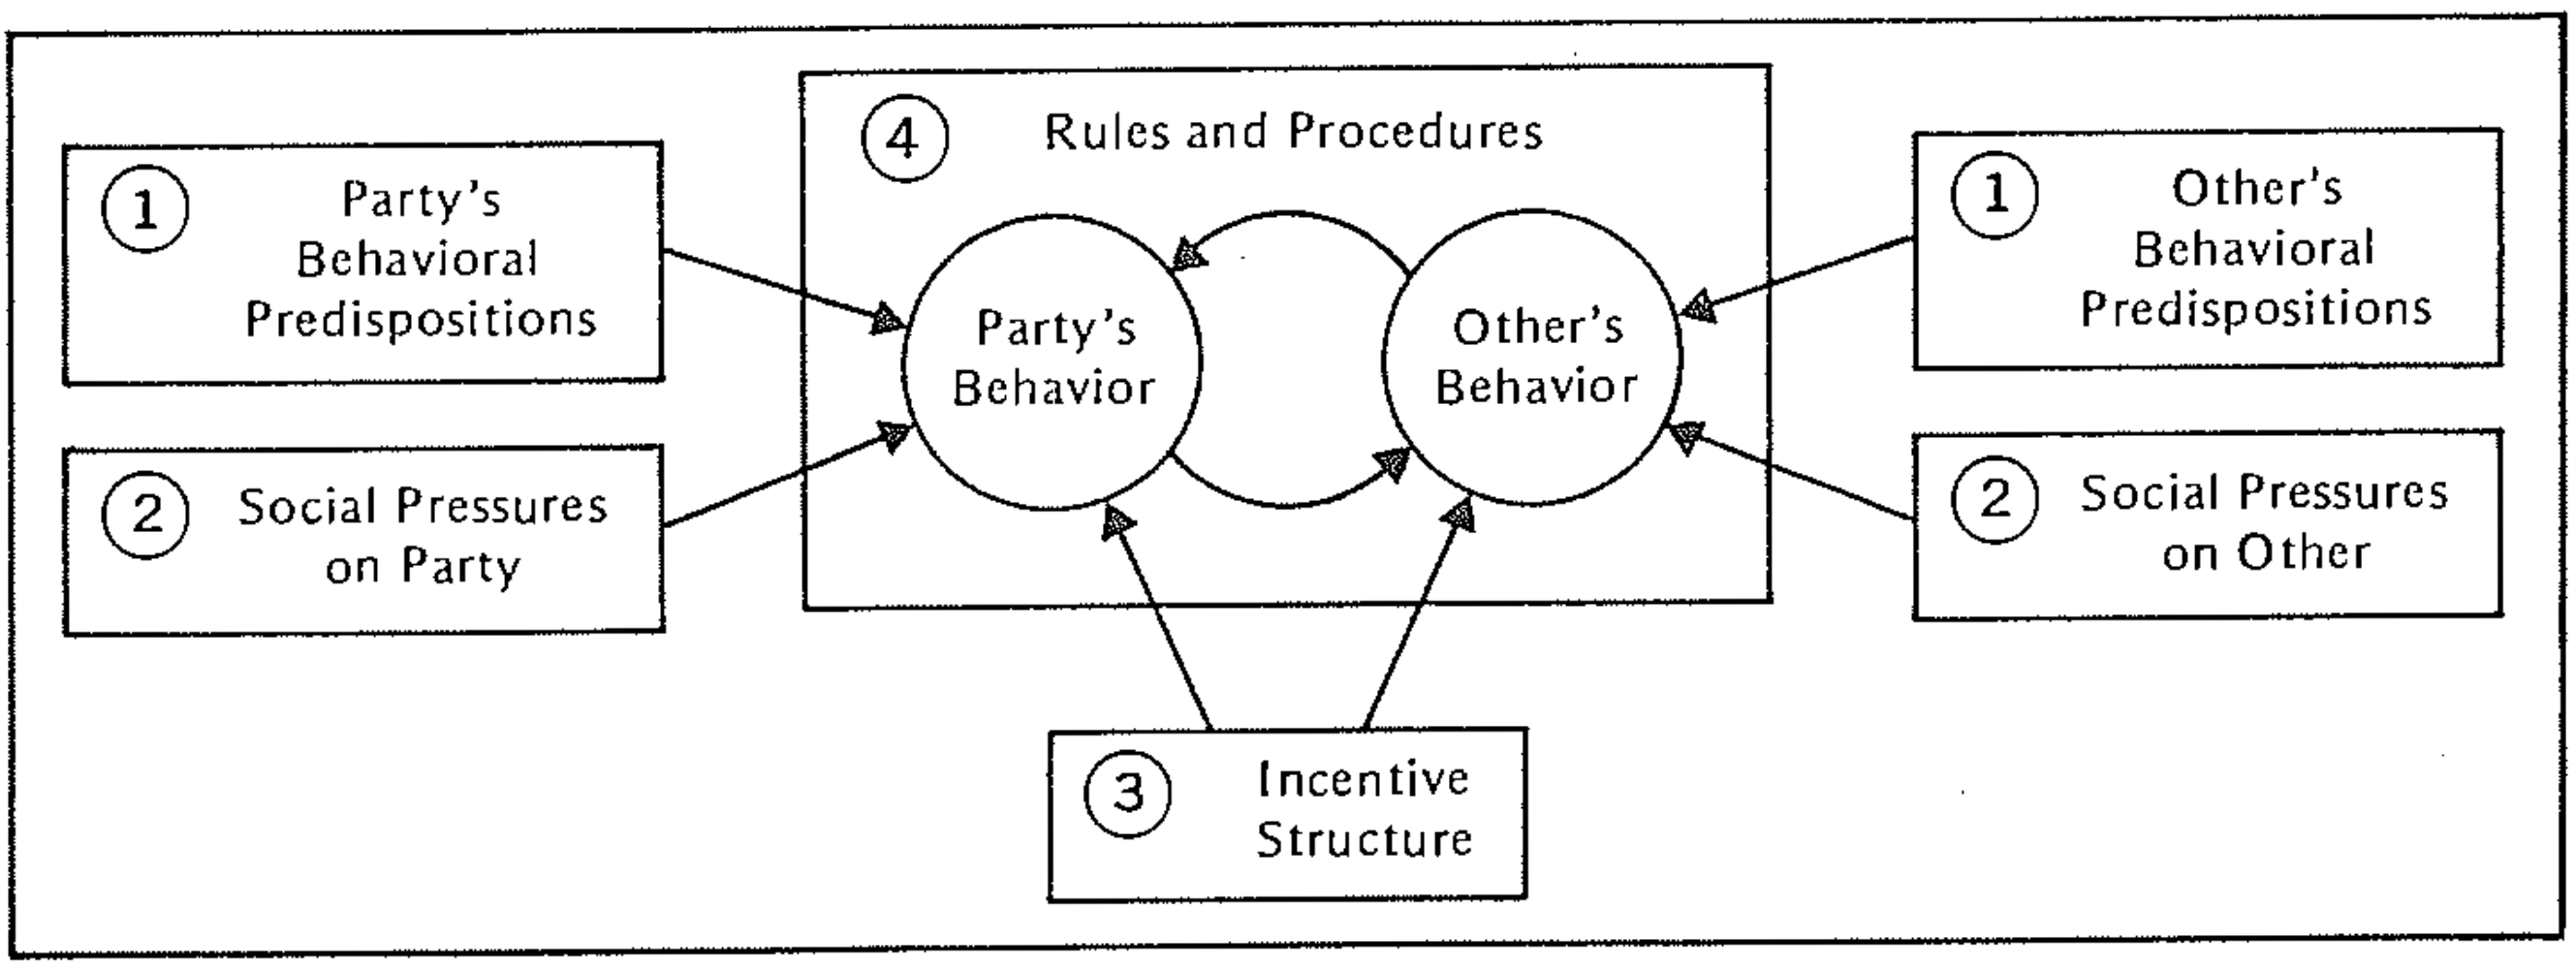
\includegraphics[width=1.0\textwidth]{images/structural_model.png}
	\end{figure}
\end{frame}

\begin{frame}
	\frametitle{Verhaltensabsichten}
	\begin{itemize}
		\item Dominanter Stil: Prim�rziel, dass erreicht werden soll
		\item Backup Stil: Falls das Prim�rziel nicht erreicht werden kann werden alternative Ziele verfolgt
	\end{itemize}
\end{frame}

\begin{frame}
	\frametitle{Sozialer Druck}
	\begin{itemize}
		\item Druck des Auftraggebers / der repr�sentierten Gruppe
		\item Umgebender sozialer Druck durch neutrale Beobachter oder kulturelle Werte 
	\end{itemize}
\end{frame}

\begin{frame}
	\frametitle{Beziehung zwischen den Interessen der Parteien}
	\begin{itemize}
		\item Abh�ngig davon, ob ein Interessenkonflikt vorliegt
		\begin{itemize}
			\item Wettbewerb: Knappe Ressourcen erm�glichen nur die Umsetzung der Interessen einer Partei
			\item Gemeinsame Probleme: F�rdert kooperatives Verhalten
			\item Kombination aus beiden
		\end{itemize}
	\end{itemize}
\end{frame}

%//Komponenten einfügen

%//Optional
\begin{frame}
	\frametitle{Zusammenfassung der Modelle}
	\begin{itemize}
		\item Prozessmodell
		\begin{itemize}
			\item Beschreibt interne Dynamik eines Konflikt als Ablauf von Phasen
			\item Phasen bilden abh�ngige Eventzyklen
		\end{itemize}
		\item Strukturmodell
		\begin{itemize}
			\item Beschreibt interne einen Konflikt als Mischung von Druck und Interessen von verschiedenen Parteien
		\end{itemize}
	\end{itemize}
\end{frame}

%//F?hrungsstile
\begin{frame}
	\frametitle{5-Punkt Modell \"Ubersicht}		
	\begin{itemize}
		\item Vermeidung \textcolor{lightgray}{(in-action)}			% Robin
		\item Machteinsatz \textcolor{lightgray}{(contending)}			% Sven
		\item Kompromiss									% Sven
		\item Anpassung \textcolor{lightgray}{(with-drawing)}			% Robin
		\item Zusammenarbeit \textcolor{lightgray}{(problem solving)}	% Sven
	\end{itemize}
\end{frame}

\begin{frame}
	\frametitle{Vermeidung}
	\begin{itemize}
		\item Konflikte werden ignoriert
		\item Bei Konfrontation: Flucht
		\item Unterscheidung von kurz- und langfristiger Vermeidung
	\end{itemize}
\end{frame}

\begin{frame}
	\frametitle{Anpassung}
	\begin{itemize}
		\item Erf�llung der W�nsche der anderen Partei ohne R�cksicht auf eigene Interessen
		\item Kann verschiedene Gr�nde haben
		\begin{itemize}
			\item Akzeptanz der (fachlichen) �berlegenheit der anderen Partei
			\item Aufbau von sozialem Kredit
			\item Gesichtswahrung bei Hinzuziehen eines Mediators
		\end{itemize}
	\end{itemize}
\end{frame}

%//Folien zu einzelnen Führungsstilen
%//Withdrawing, inaction: Robin
%//Others: Sven

%//Jeder remote sein Zeug
%//Fazit Folie

\end{document}
